In this chapter, results obtained by feature selection and modeling are shown with respect for each different period, resolution and target variable. 

\section{Case of Study}
This case of study aims to discover the main factors which affects mostly the target variable chosen. In order to examine the behavior of each variable in a data set over time, several grid data are collected, each one with different resolution, period and configuration (\href{fig:test_params}):
\subsection{Data sets description}
\subsubsection{Period}  
Data collected are dated 2021 because are the most recent and, with respect 2020, the ones not particularly affecting by emission reduction caused by lockdown for COVID-19 pandemic\cite{bontempi2022analysis}. In this case of study grid data are chosen by considering the effect of intensive agriculture, with these particular condition:
    \begin{itemize}
        \item In order to have right condition for farming, in the period chosen the terrain shouldn't be frozen (Temperature > 0°C). So I selected data coming from spring, summer and autumn period (discarding winter);
        \item For better highlighting the effect of intense agriculture with the usage of fertilizer and pesticides, which are the main pollution emission factors, weeks preceding a rain period are selected;
\end{itemize}
In this way, several grid data are chosen from 5 different weeks:
\begin{itemize}
    \item 24 March - 31 March 2021;
    \item 18 April - 25 April 2021;
    \item 17 July - 24 July 2021;
    \item 3 September - 10 September 2021;
    \item 7 October - 14 October 2021
\end{itemize}
\subsubsection{Resolutions}
0.1° ($\sim$ 10km) and 0.01° ($\sim$ 1km) resolutions are selected for the grid data. For increasing the number of observation provided by the limited ARPA stations in Lombardy a k-nearest neighbors algorithm is applied to adding the buffer of values (with k respectively equal to 10 and 30 for each resolution). Then, the value added are computed using the RBF interpolation (as already explained in the \hyperref[sec:Data cleaning]{Data Cleaning section}.

\subsubsection{Target Variables}
PM25 and ammonia (NH3) provided by ARPA sensors are the one chosen as target variables('pm25\_st' and 'nh3\_st'). I chose them because are strictly related between them and are the most related to intense farming pollution.
ARPA air quality monitoring stations, which, operating 24 h a day 365 days a year, are periodically checked and subject to maintenance, for ensuring the proper functioning and reliability.


\subsubsection{Mountains}
Another important parameter configuration used is to filter or not the cell covered by mountains or not (climate zone = 1/2/3 of Alpes and Prealpes). In this way the test run can take in consideration or not only urban and land areas, which are more affected by air pollution phenomena.


\subsubsection{Feature Selection}
\label{subsub:fs}
After the preprocessing phase, I use 2 different configuration for training ML models:
\begin{itemize}
    \item Using the set of variables selected for each different period;
    \item Using a general set of variables. This was computed by averaging the feature selected for each different period with Borda Count another time;
\end{itemize}
Before this phase, using the VarianceThreshold class, variables with variance less than 0.2 were discarded. 

\begin{figure}
    \centering
    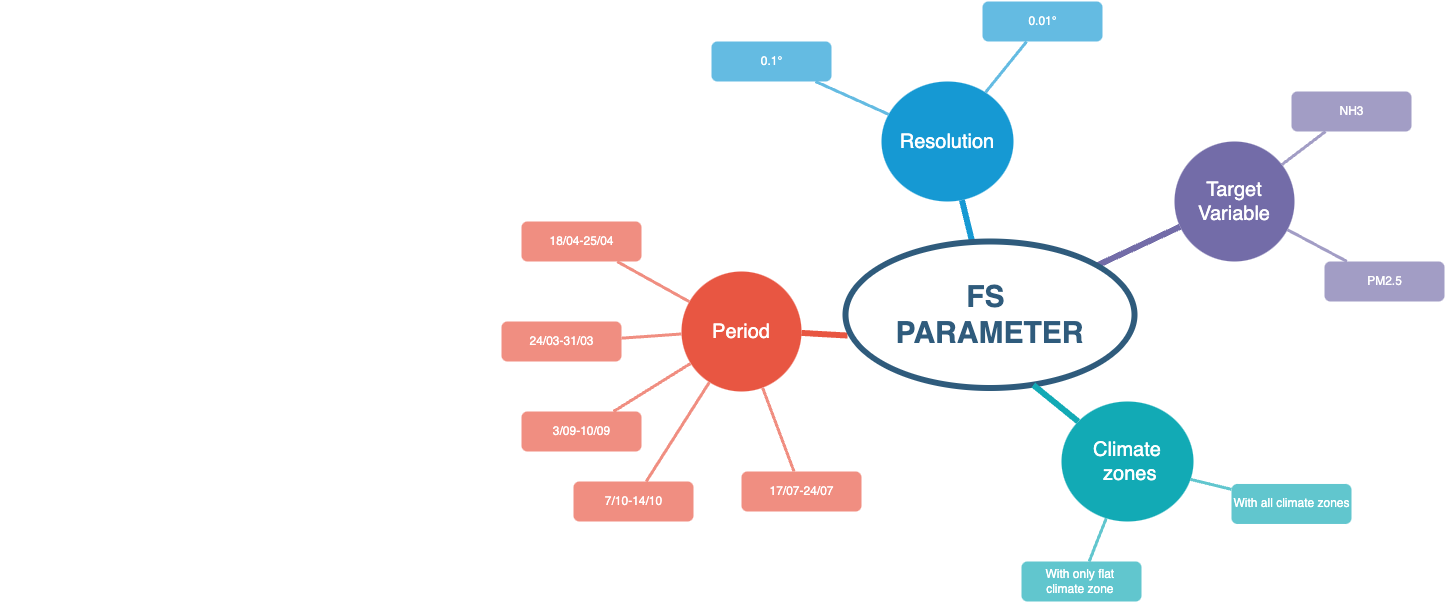
\includegraphics[width=.9\textwidth]{src/images/test_param.png}
    \caption{Parameter taken in consideration for tests execution.}
    \label{fig:test_params}
\end{figure}
-data
-motivazioni
-risoluzioni
-parametri test
\section{FS Results with target variable = 'pm25\_st'}
\label{sec:pm25}
\subsection{Resolution = 0.01°}
\subsubsection{Including mountains}
\begin{center}
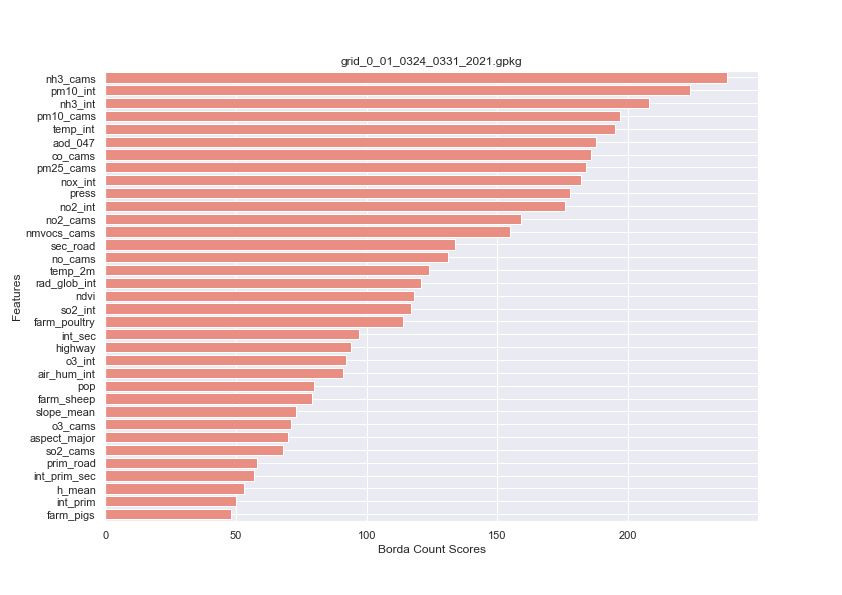
\includegraphics[width=0.9\textwidth]{images/fs_results/pm25/001/montains/grid_0_01_0324_0331_2021.png}
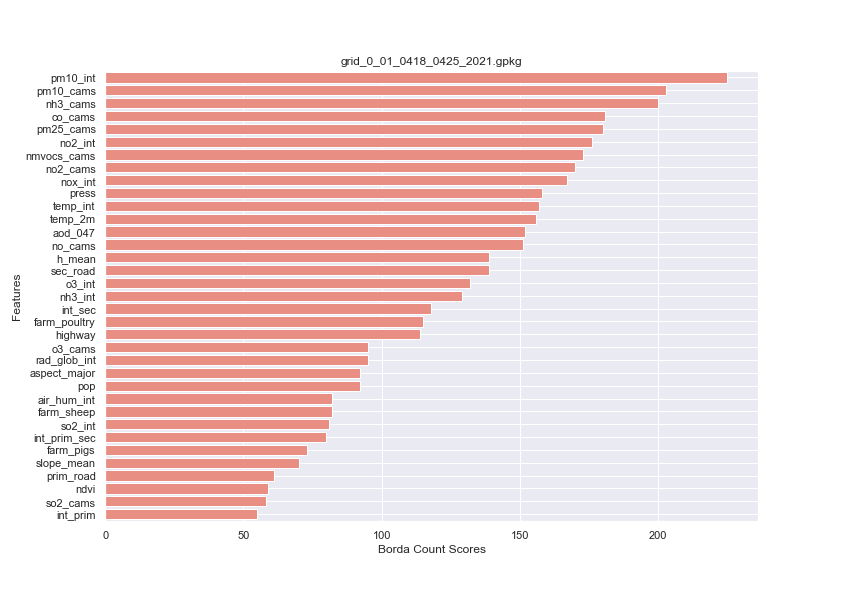
\includegraphics[width=0.9\textwidth]{images/fs_results/pm25/001/montains/grid_0_01_0418_0425_2021.png}
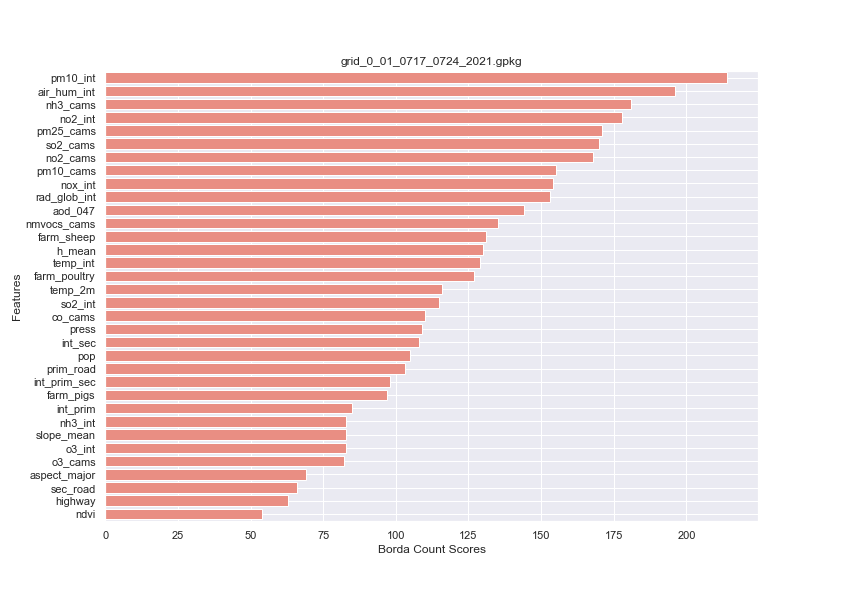
\includegraphics[width=.9\textwidth]{images/fs_results/pm25/001/montains/grid_0_01_0717_0724_2021.png}
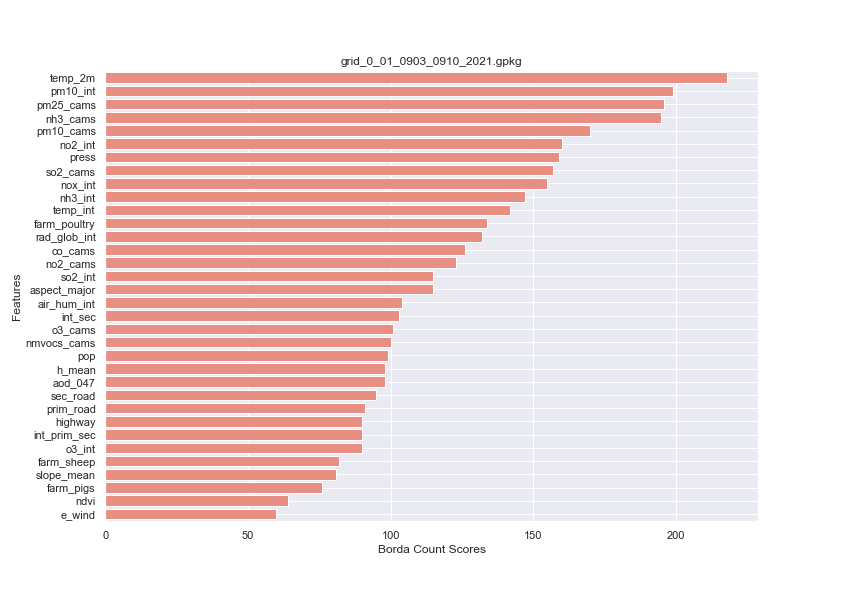
\includegraphics[width=.9\textwidth]{images/fs_results/pm25/001/montains/grid_0_01_0903_0910_2021.png}
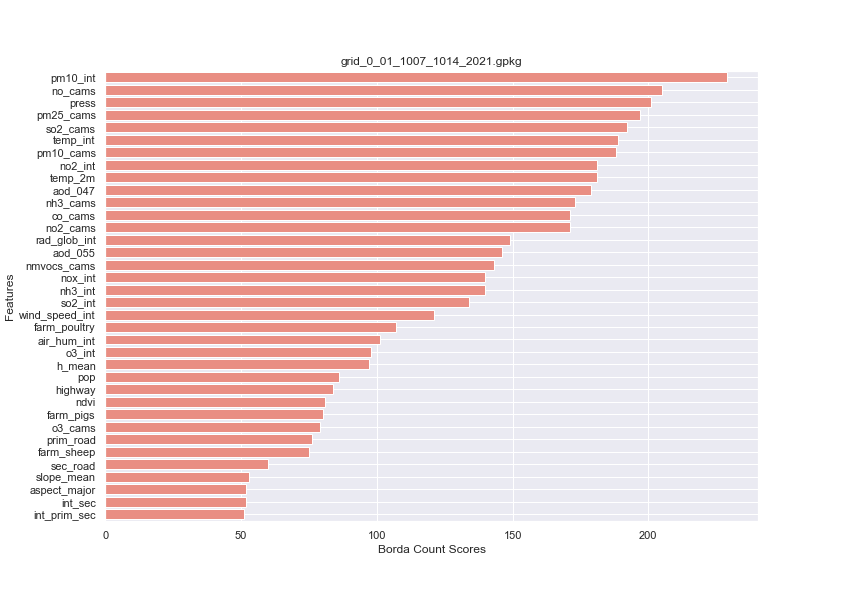
\includegraphics[width=.9\textwidth]{images/fs_results/pm25/001/montains/grid_0_01_1007_1014_2021.png}
\end{center}

\subsubsection{Excluding mountains}
\begin{center}
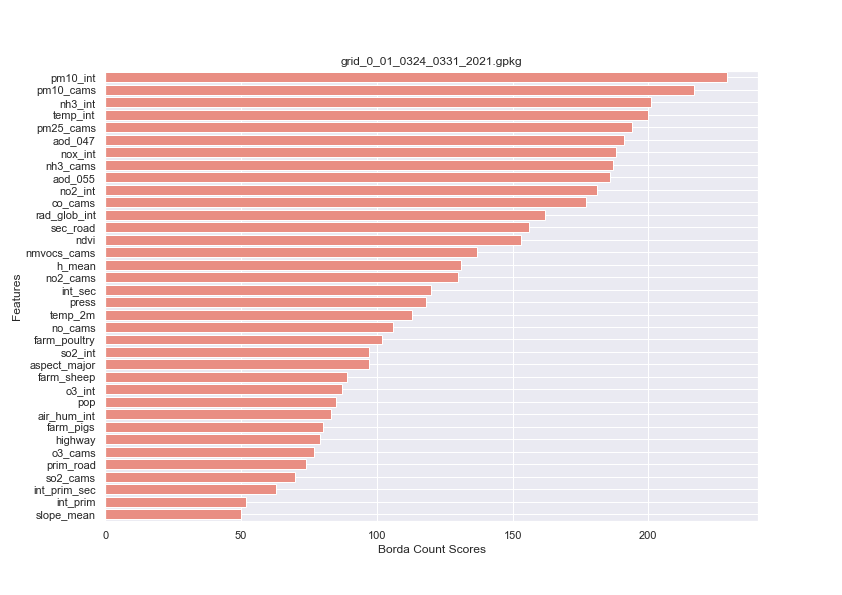
\includegraphics[width=.9\textwidth]{images/fs_results/pm25/001/no_montains/grid_0_01_0324_0331_2021.png}
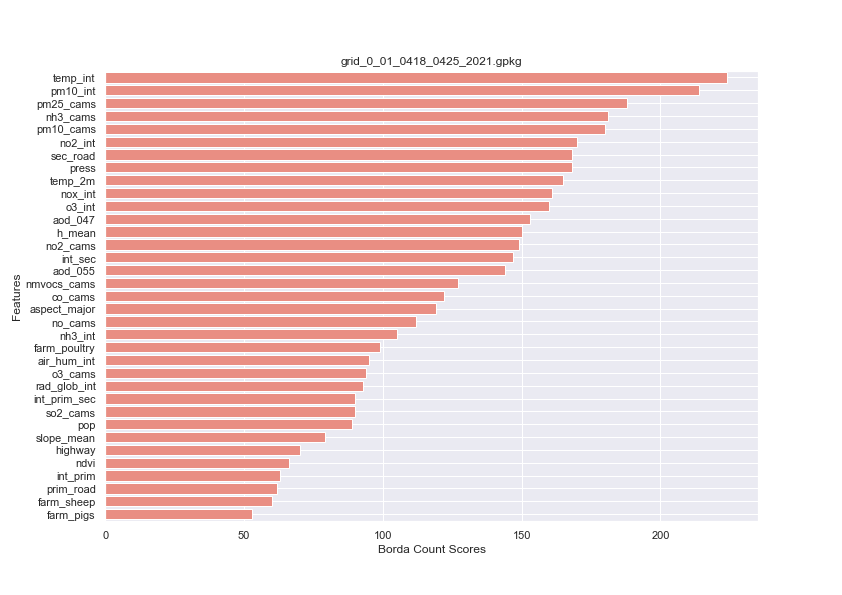
\includegraphics[width=.9\textwidth]{images/fs_results/pm25/001/no_montains/grid_0_01_0418_0425_2021.png}
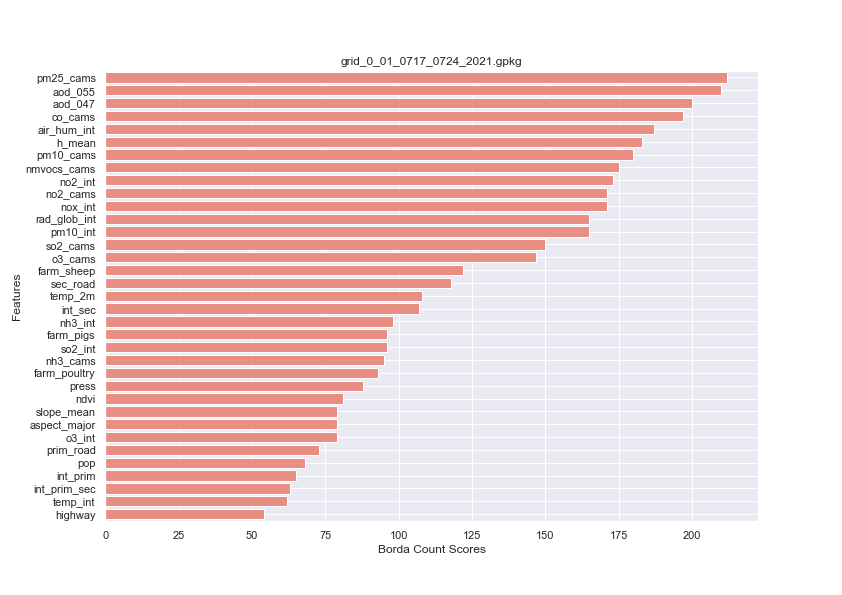
\includegraphics[width=.9\textwidth]{images/fs_results/pm25/001/no_montains/grid_0_01_0717_0724_2021.png}
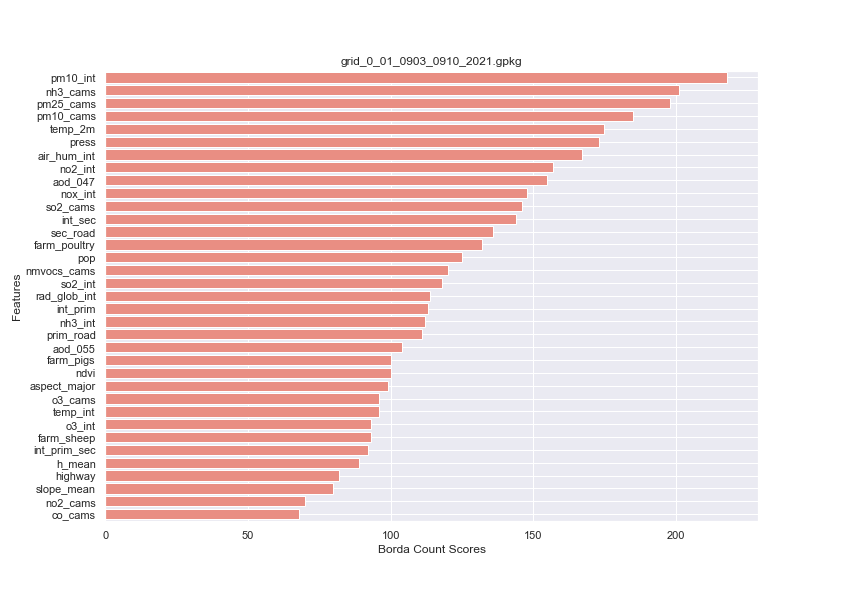
\includegraphics[width=.9\textwidth]{images/fs_results/pm25/001/no_montains/grid_0_01_0903_0910_2021.png}
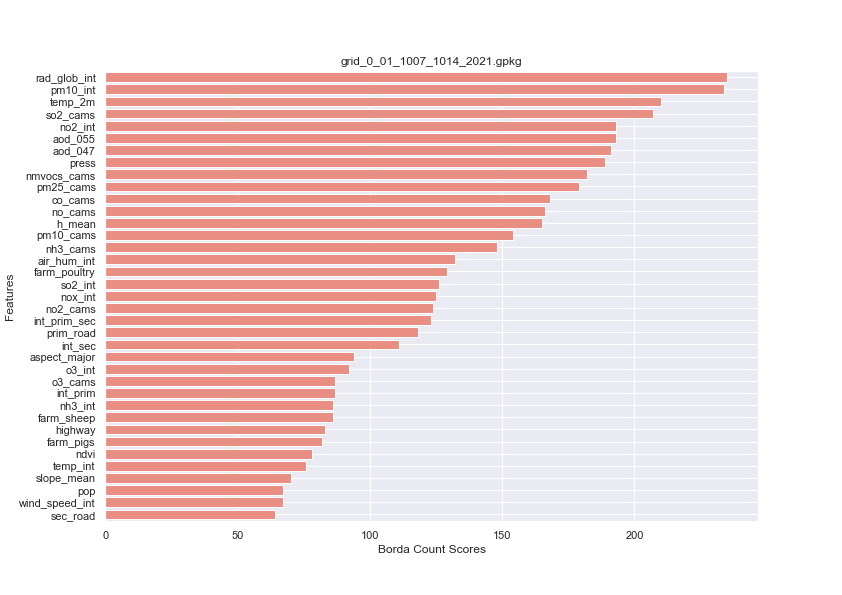
\includegraphics[width=.9\textwidth]{images/fs_results/pm25/001/no_montains/grid_0_01_1007_1014_2021.png}
\end{center}
\subsection{Resolution = 0.1°}
\subsubsection{Including mountains}
\begin{center}
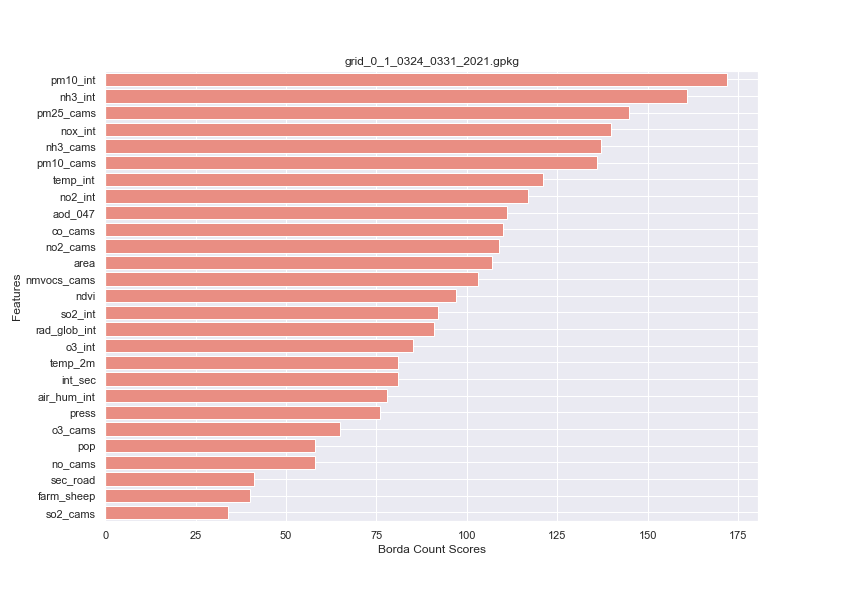
\includegraphics[width=0.9\textwidth]{images/fs_results/pm25/01/montains/grid_0_1_0324_0331_2021.png}
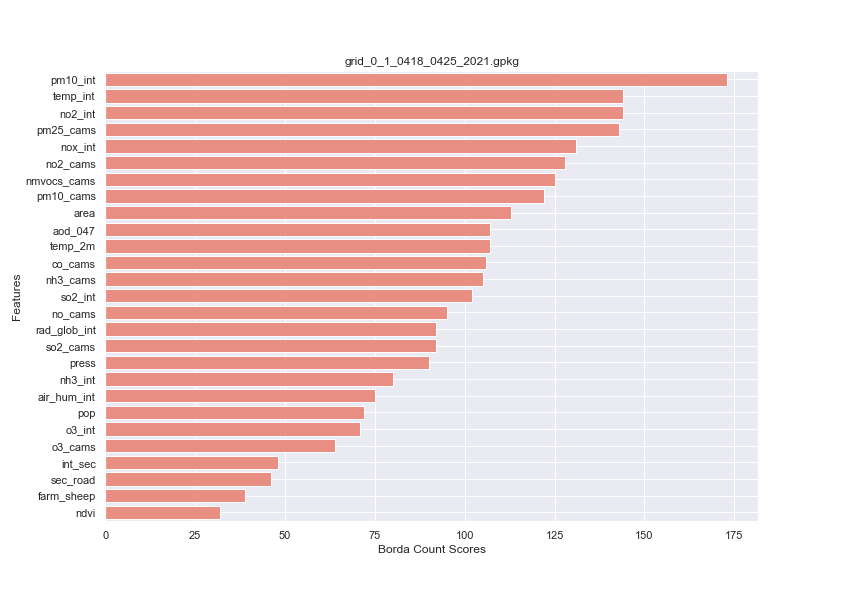
\includegraphics[width=0.9\textwidth]{images/fs_results/pm25/01/montains/grid_0_1_0418_0425_2021.png}
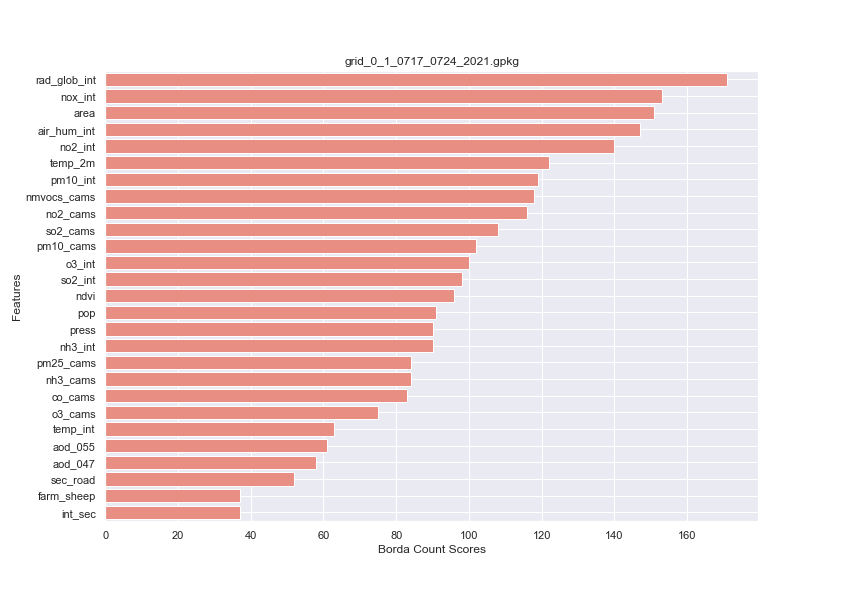
\includegraphics[width=.9\textwidth]{images/fs_results/pm25/01/montains/grid_0_1_0717_0724_2021.png}
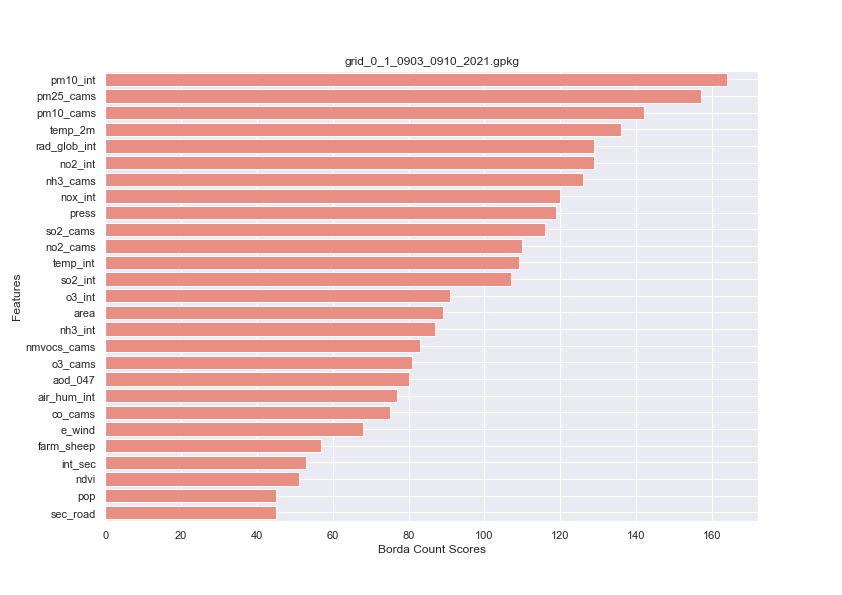
\includegraphics[width=.9\textwidth]{images/fs_results/pm25/01/montains/grid_0_1_0903_0910_2021.png}
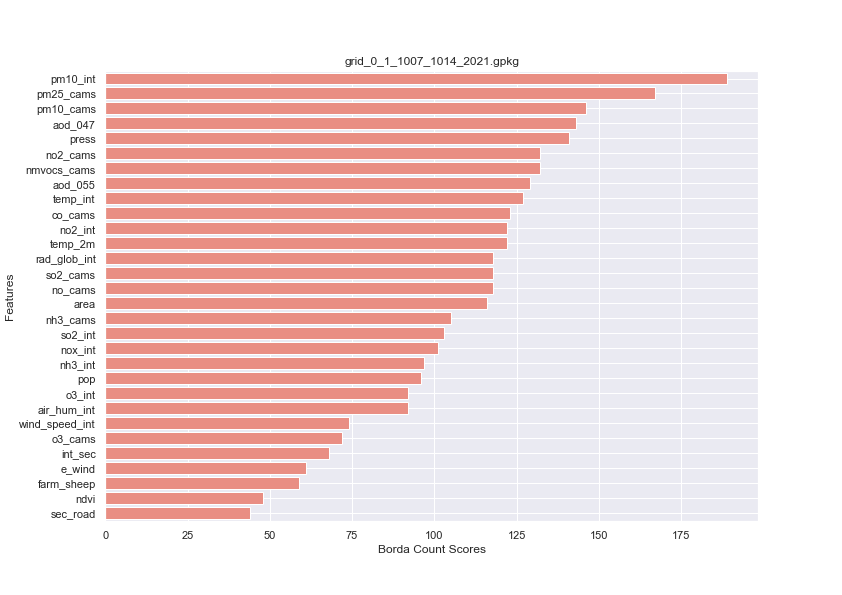
\includegraphics[width=.9\textwidth]{images/fs_results/pm25/01/montains/grid_0_1_1007_1014_2021.png}
\end{center}

\subsubsection{Excluding mountains}
\begin{center}
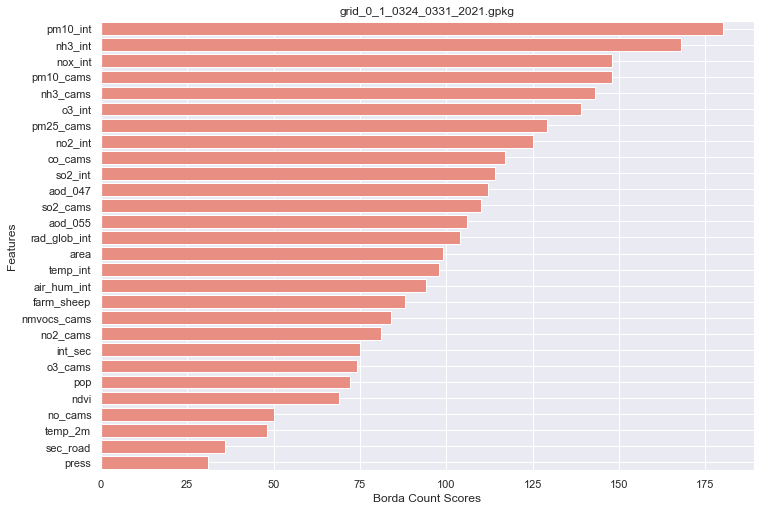
\includegraphics[width=.9\textwidth]{images/fs_results/pm25/01/no_montains/grid_0_1_0324_0331_2021.png}
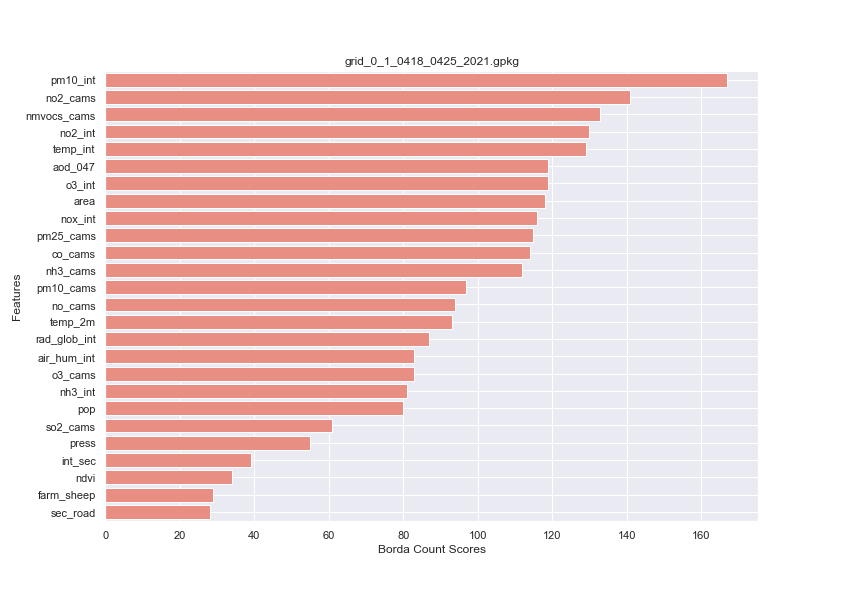
\includegraphics[width=.9\textwidth]{images/fs_results/pm25/01/no_montains/grid_0_1_0418_0425_2021.png}
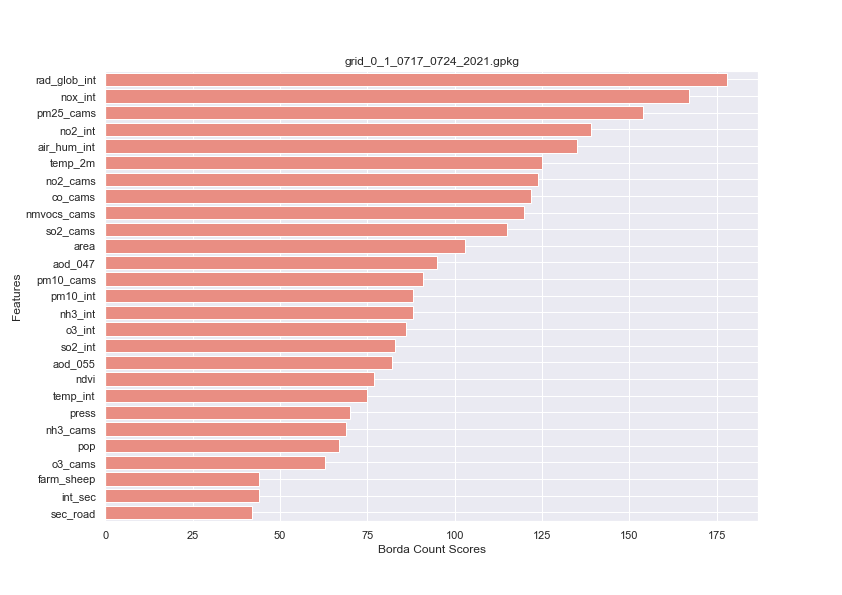
\includegraphics[width=.9\textwidth]{images/fs_results/pm25/01/no_montains/grid_0_1_0717_0724_2021.png}
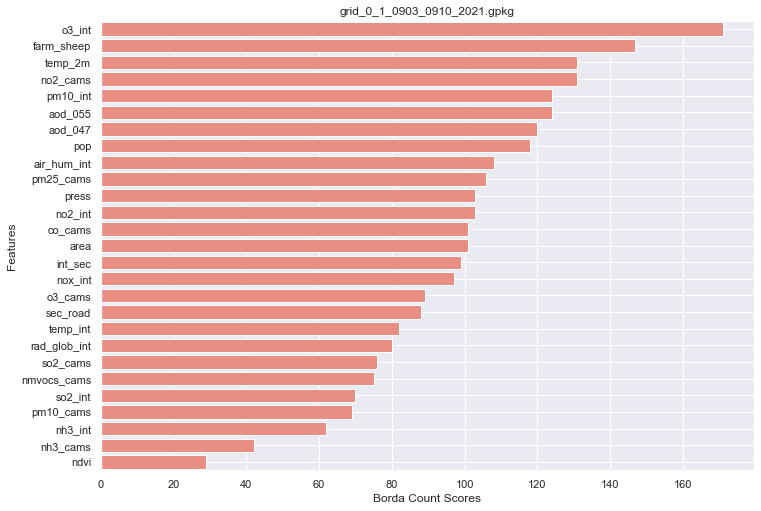
\includegraphics[width=.9\textwidth]{images/fs_results/pm25/01/no_montains/grid_0_1_0903_0910_2021.png}
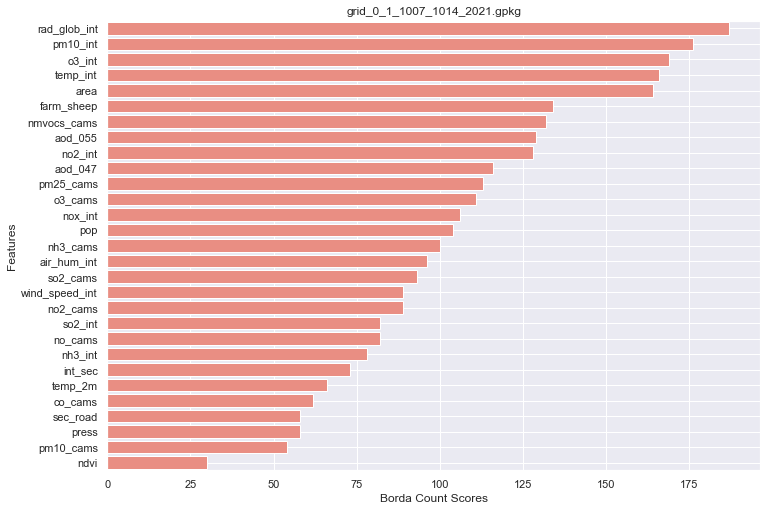
\includegraphics[width=.9\textwidth]{images/fs_results/pm25/01/no_montains/grid_0_1_1007_1014_2021.png}
\end{center}

\section{FS Results with target variable = 'nh3\_st'  }
\subsection{Resolution = 0.1°}
\subsubsection{Including mountains}
\begin{center}
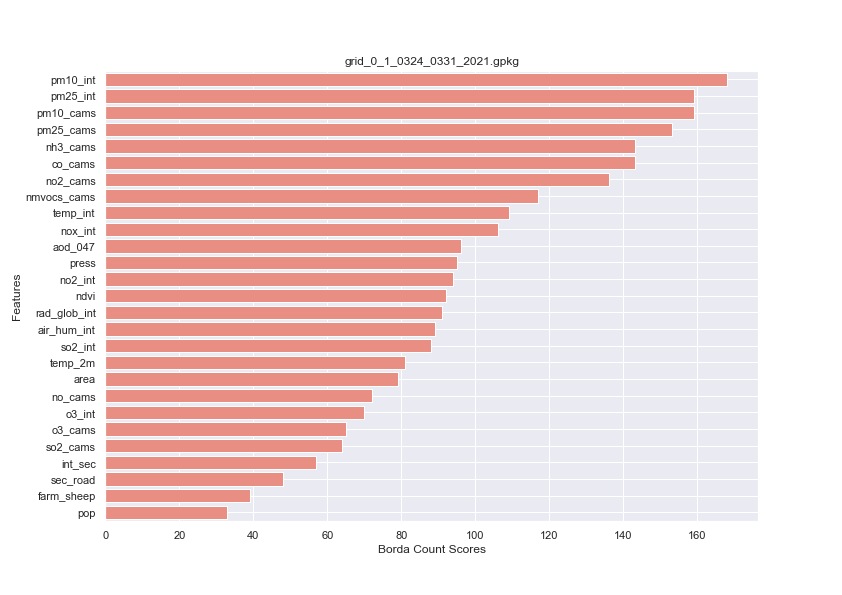
\includegraphics[width=0.9\textwidth]{images/fs_results/nh3/01/montains/grid_0_1_0324_0331_2021.png}
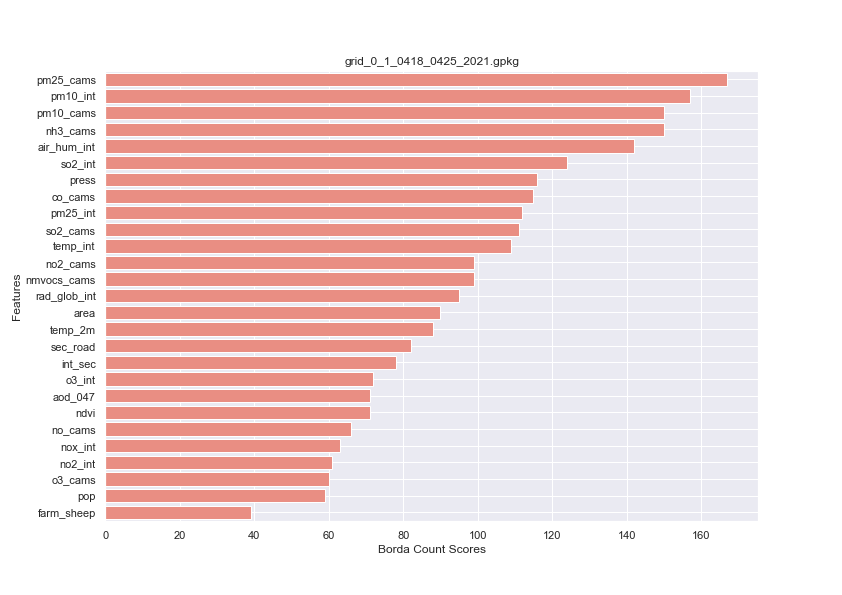
\includegraphics[width=0.9\textwidth]{images/fs_results/nh3/01/montains/grid_0_1_0418_0425_2021.png}
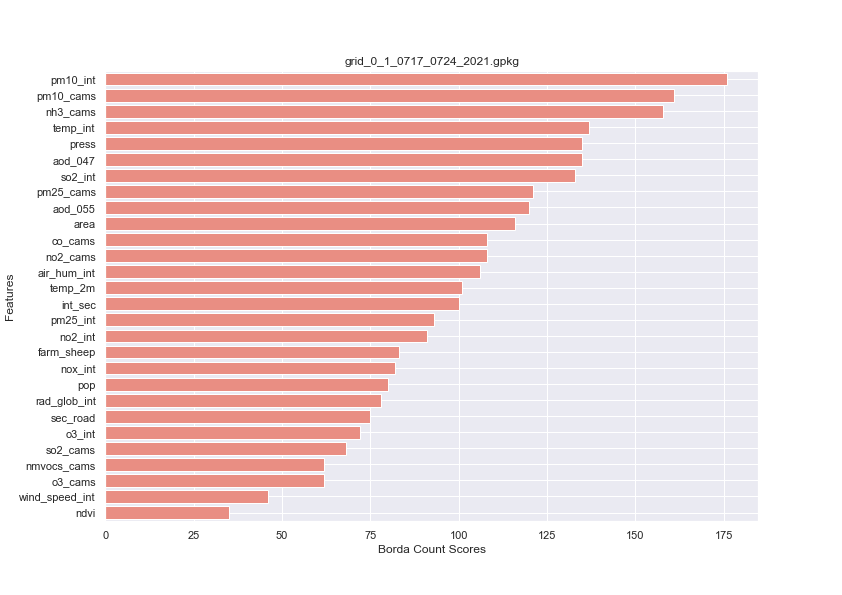
\includegraphics[width=.9\textwidth]{images/fs_results/nh3/01/montains/grid_0_1_0717_0724_2021.png}
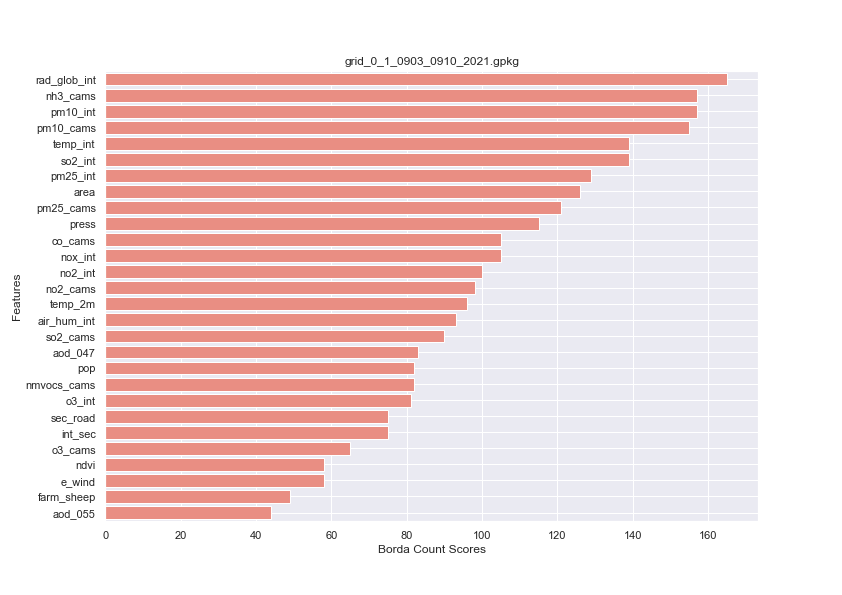
\includegraphics[width=.9\textwidth]{images/fs_results/nh3/01/montains/grid_0_1_0903_0910_2021.png}
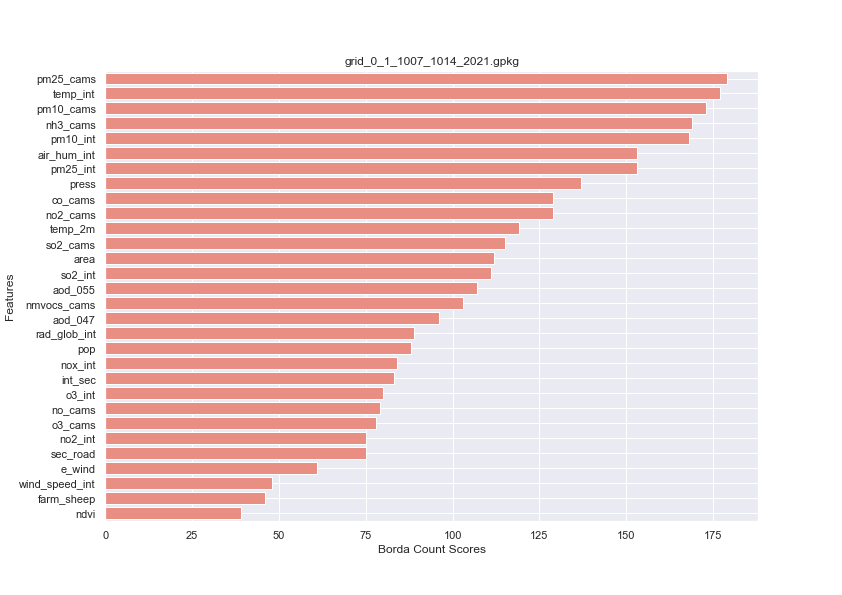
\includegraphics[width=.9\textwidth]{images/fs_results/nh3/01/montains/grid_0_1_1007_1014_2021.png}
\end{center}

\subsubsection{Excluding mountains}
\begin{center}
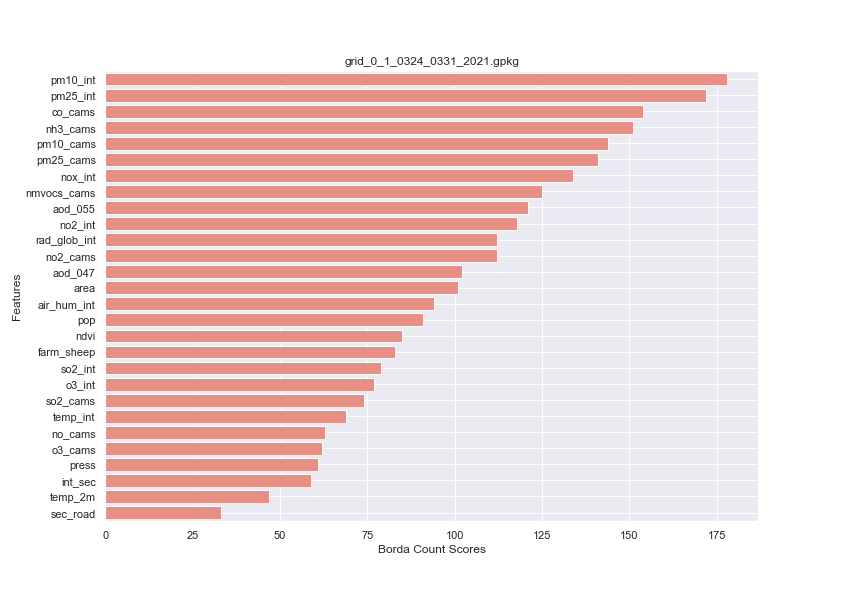
\includegraphics[width=.9\textwidth]{images/fs_results/nh3/01/no_montains/grid_0_1_0324_0331_2021.png}
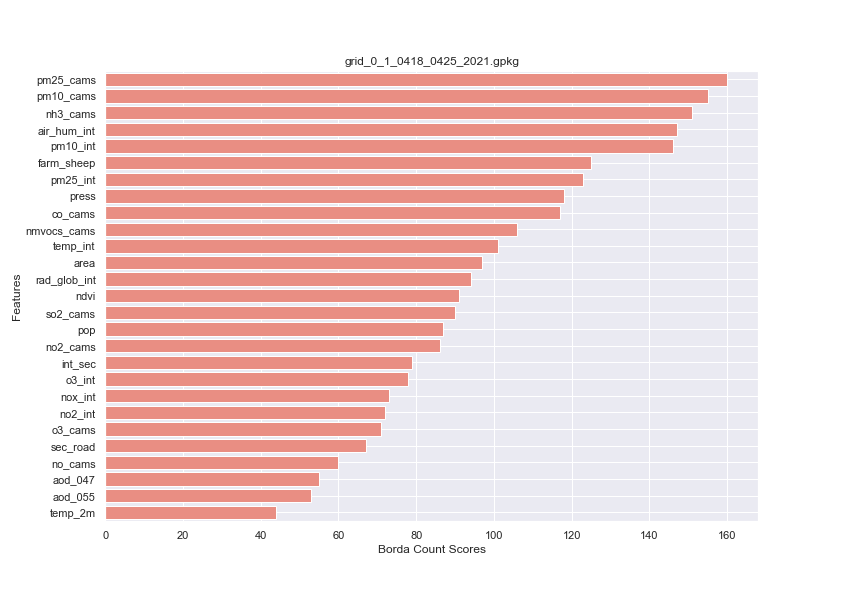
\includegraphics[width=.9\textwidth]{images/fs_results/nh3/01/no_montains/grid_0_1_0418_0425_2021.png}
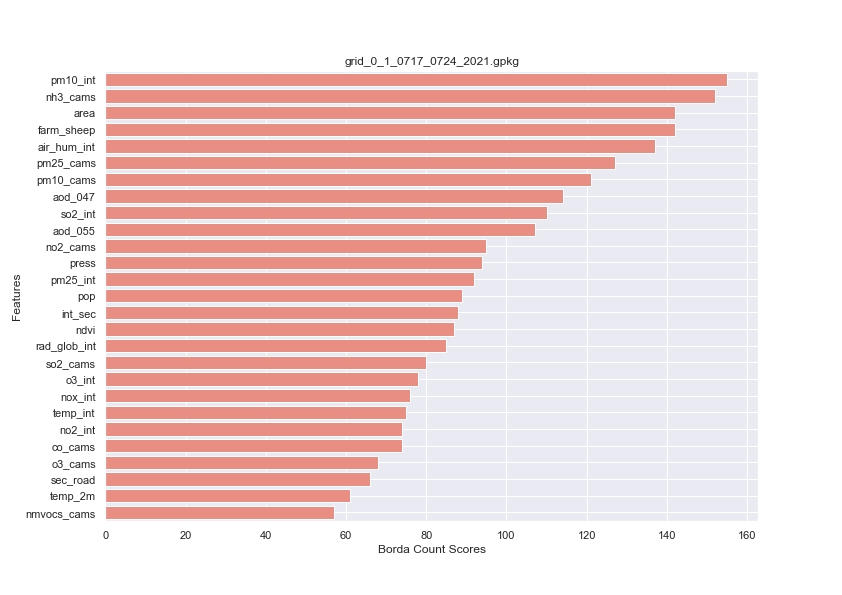
\includegraphics[width=.9\textwidth]{images/fs_results/nh3/01/no_montains/grid_0_1_0717_0724_2021.png}
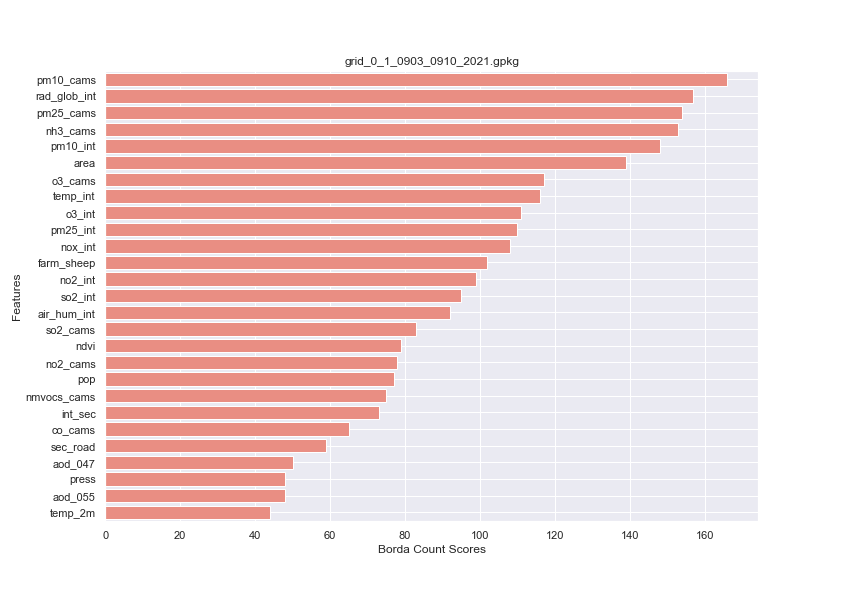
\includegraphics[width=.9\textwidth]{images/fs_results/nh3/01/no_montains/grid_0_1_0903_0910_2021.png}
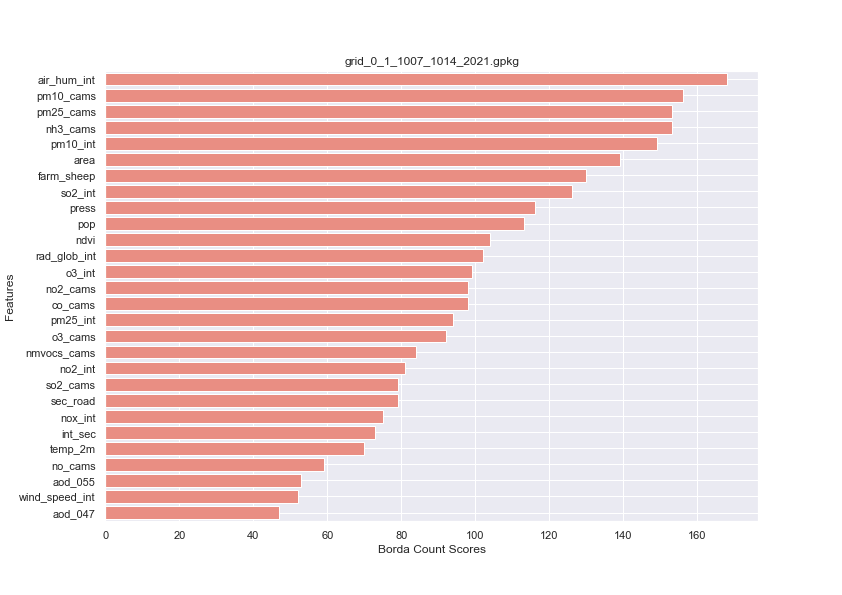
\includegraphics[width=.9\textwidth]{images/fs_results/nh3/01/no_montains/grid_0_1_1007_1014_2021.png}
\end{center}


\subsection{Resolution = 0.01°}
\subsubsection{Including mountains}
\begin{center}
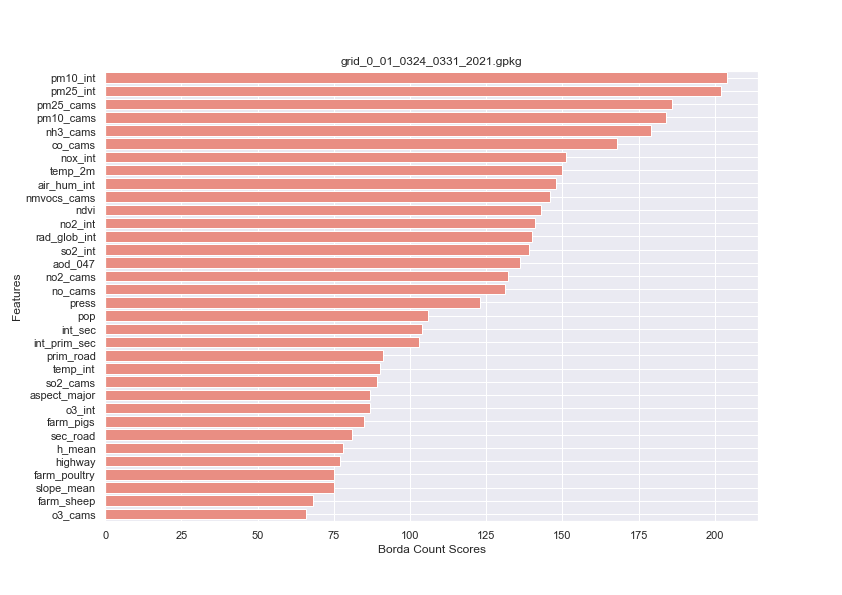
\includegraphics[width=0.9\textwidth]{images/fs_results/nh3/001/montains/grid_0_01_0324_0331_2021.png}
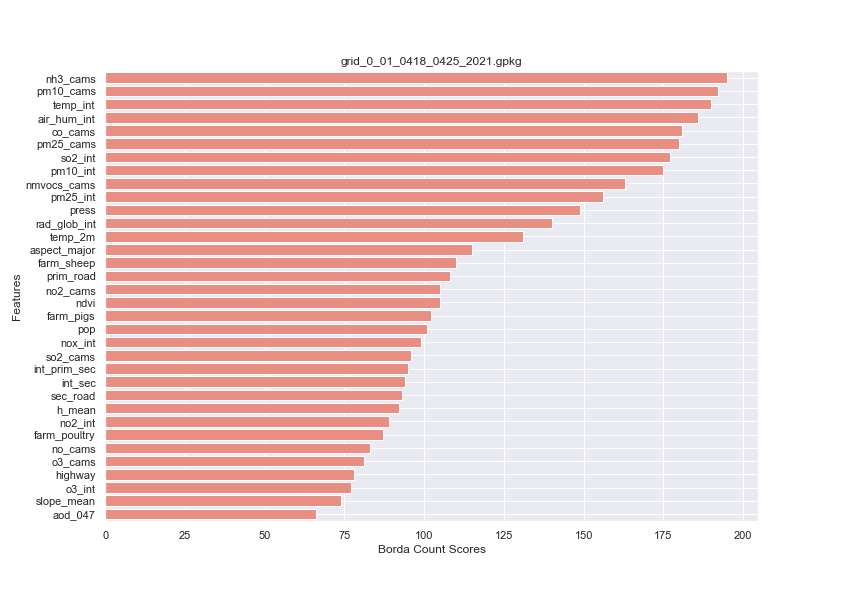
\includegraphics[width=0.9\textwidth]{images/fs_results/nh3/001/montains/grid_0_01_0418_0425_2021.png}
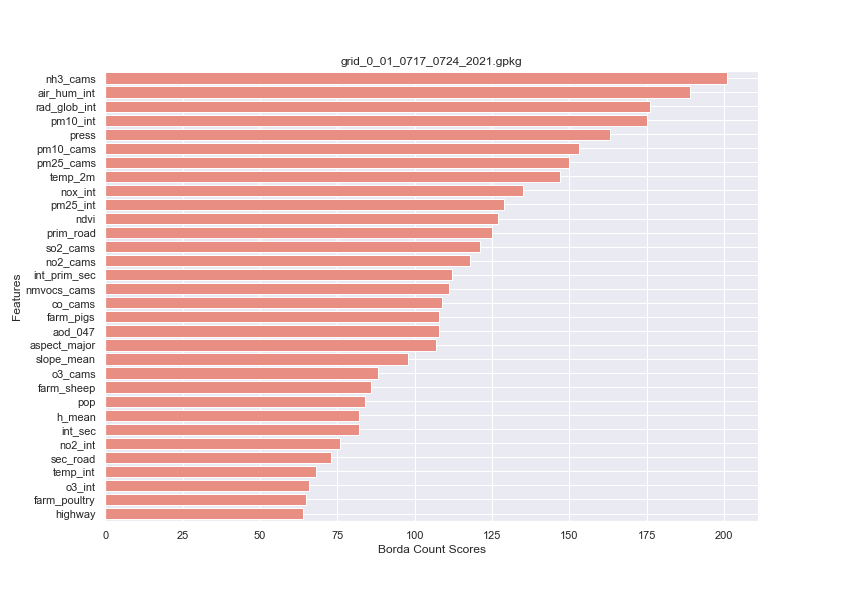
\includegraphics[width=.9\textwidth]{images/fs_results/nh3/001/montains/grid_0_01_0717_0724_2021.png}
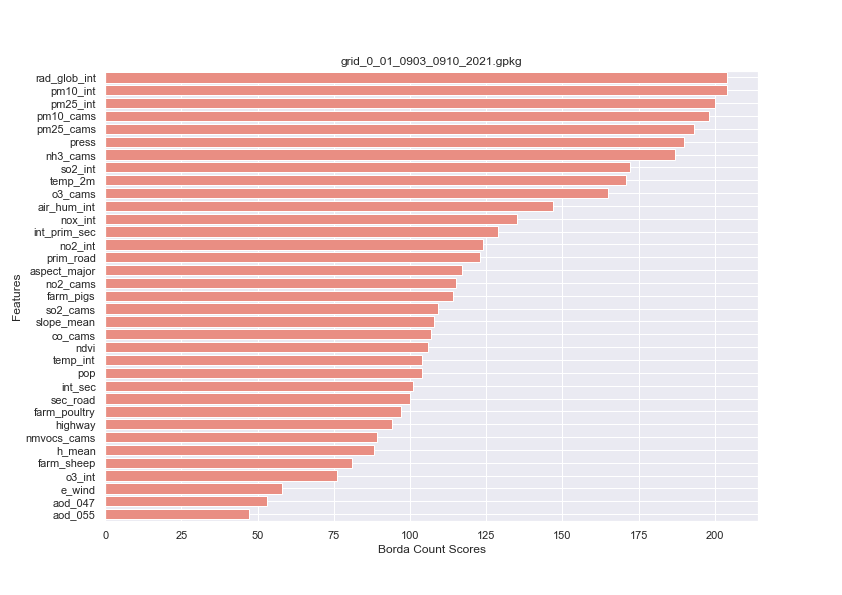
\includegraphics[width=.9\textwidth]{images/fs_results/nh3/001/montains/grid_0_01_0903_0910_2021.png}
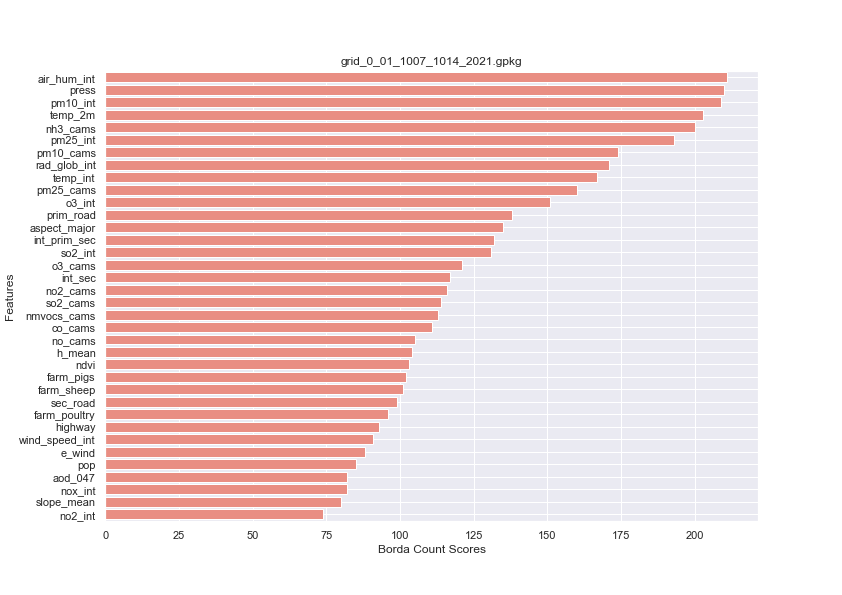
\includegraphics[width=.9\textwidth]{images/fs_results/nh3/001/montains/grid_0_01_1007_1014_2021.png}
\end{center}

\subsubsection{Excluding mountains}
\begin{center}
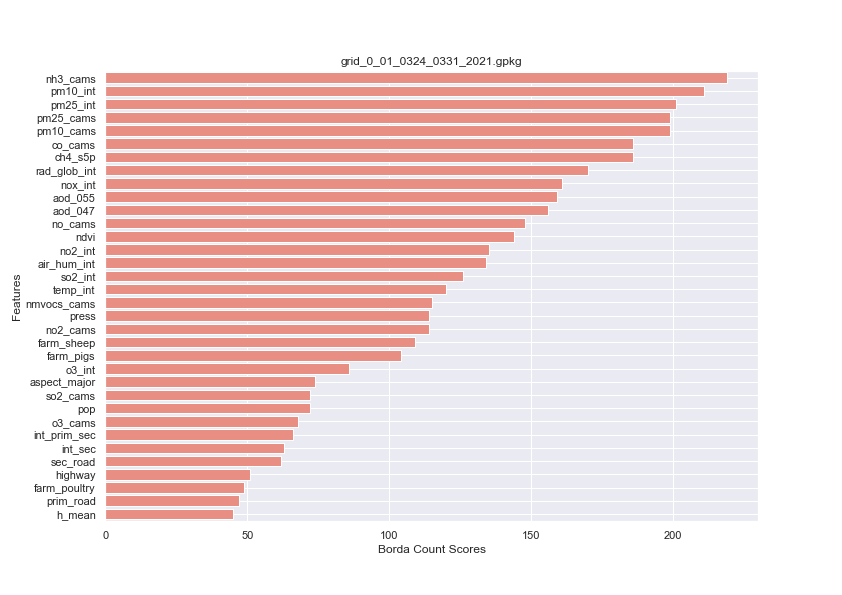
\includegraphics[width=.9\textwidth]{images/fs_results/nh3/001/no_montains/grid_0_01_0324_0331_2021.png}
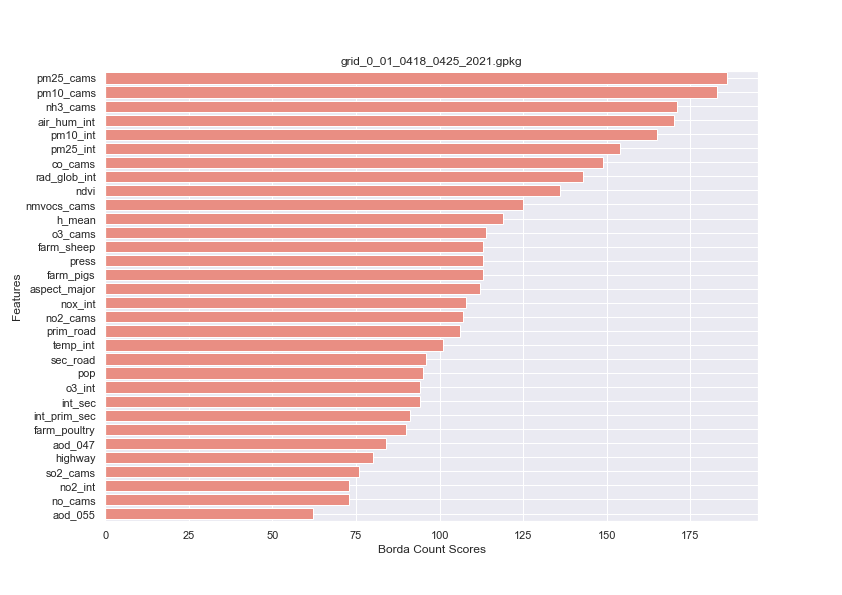
\includegraphics[width=.9\textwidth]{images/fs_results/nh3/001/no_montains/grid_0_01_0418_0425_2021.png}
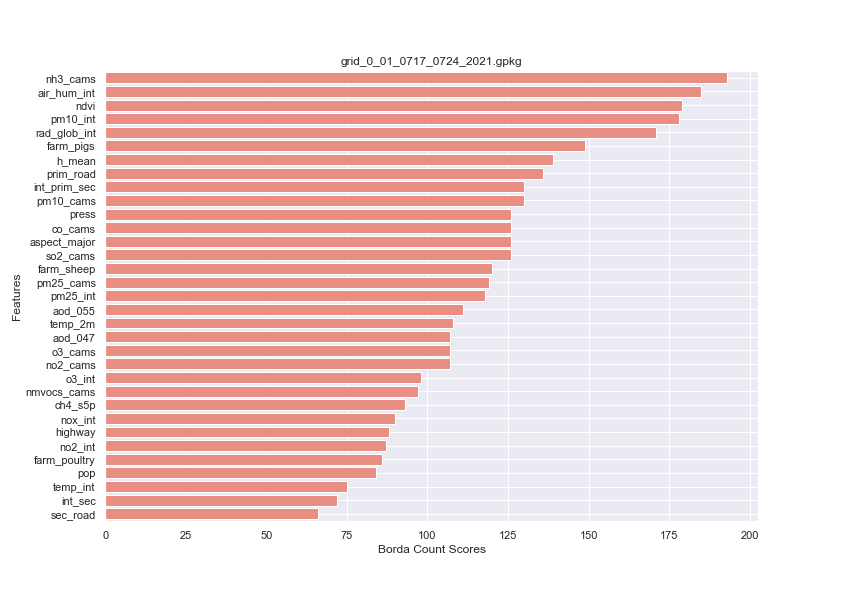
\includegraphics[width=.9\textwidth]{images/fs_results/nh3/001/no_montains/grid_0_01_0717_0724_2021.png}
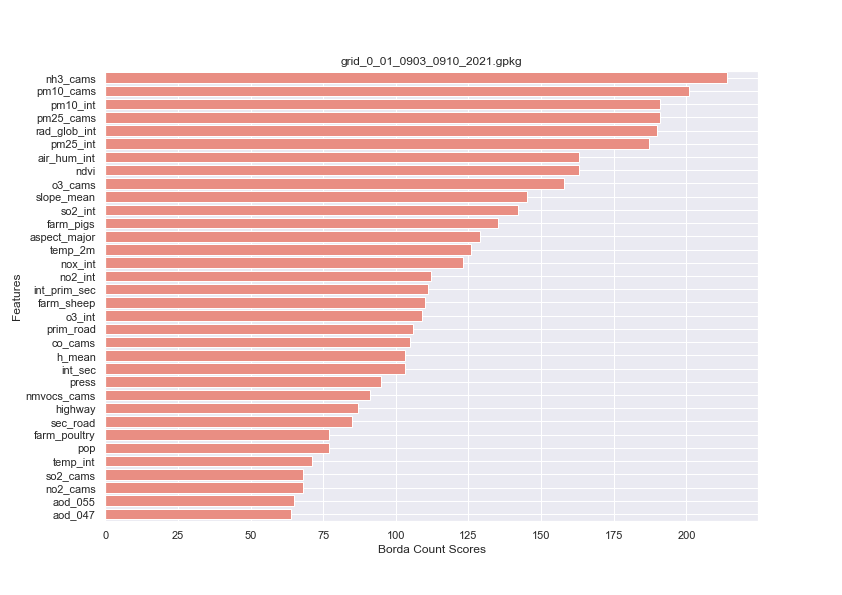
\includegraphics[width=.9\textwidth]{images/fs_results/nh3/001/no_montains/grid_0_01_0903_0910_2021.png}
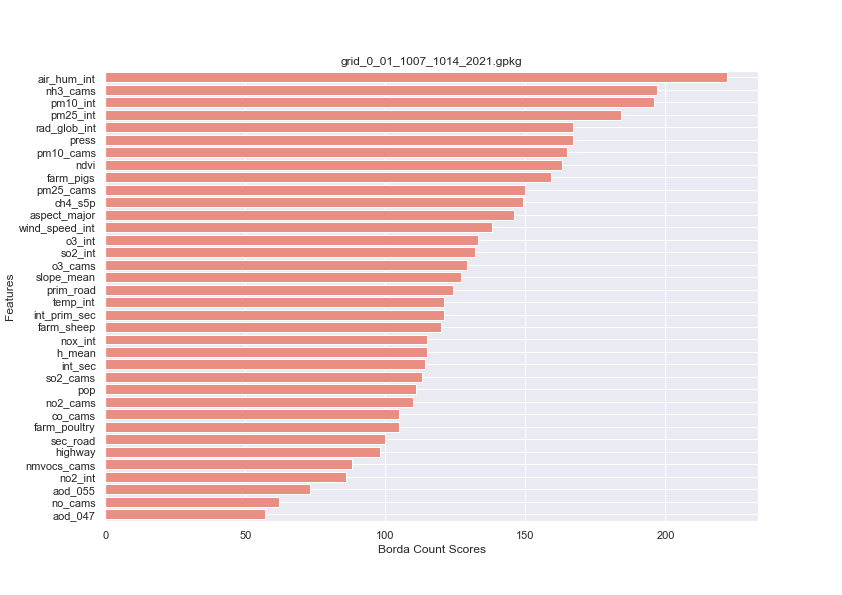
\includegraphics[width=.9\textwidth]{images/fs_results/nh3/001/no_montains/grid_0_01_1007_1014_2021.png}
\end{center}
\section{Interpretation of FS results}
In this section the results obtained for each target variable selected are explained in relation to the votes received and the positive or negative correlation assumed in the filter methods.\\
Similarity between the 2 test set are visible for many factors that influence both particulate matter and ammonia.
For instance, DTM average elevation and slope ('h\_mean' and 'slope\_mean' respectively) received many votes in both case, since air pollution affect more urban than mountain areas.

\subsection{PM25 as target variable}
Fine particulate matter (PM2.5) is one of the most common air pollutant in our environment. 
It primarily comes from transport vehicle (such as car, truck and bus), industry, burning of fuels and household activities.\\ \par
During the 5 periods, it's shown that PM25, as the other pollutants, change over the time. Air pollution change accordingly to the type of climate and atmospheric conditions.\\
Air pollution analysis can confirm the presence of high quantity in winter and heating season and low in summer months\cite{cichowicz2017dispersion}. This is not applied to the ozone ('o3\_int' and 'o3\_cams'), which should be, on the contrary, higher during summer due to combination of heat and sunlight which reacts with nitrogen oxides (NOx) and volatile organic compounds. But for the week between 17 and 24 July a negative correlation between them is found, on the contrary with respect to certain studies found in literature\cite{zhu2019correlations}\cite{biglari2017relationship}.\\
In the tests is also visible the score obtained by ozone ('o3\_int') which tends to be positively correlated in the period between 18 and 25 April.\\
This, as mentioned before, is possibly due to their common precursors, such as nitrogen oxides and volatile organic compounds and their simultaneous generation in photochemical reactions. Indeed, in the given period both ('nox\_int' and 'nmvocs\_int') have a positive correlation and an high number votes.\\
By the bar plots attached in the first \hyperref[sec:pm25]{section}, the most correlated variables to PM25 belong mostly to pollutant. In particular PM10 provided by ARPA and CAMS, in the various test executed is one of the most correlated pollutant. Indeed, 'pm10\_int' and 'pm10\_cams' have always a number votes between 150 and 240. Strong positive correlation between PM25 and PM10 is also proved in literature\cite{zhou2016concentrations}. 
Other pollutants with an high significant number of votes (greater than 100) are nitrogen dioxide ('no2\_int'), nitrogen monoxide ('no\_int'), sulphur dioxide('so2\_int' and 'so2\_cams') and aerosol optical depth ('aod\_047' and 'aod\_055'). It's evident that this pollutants have a strong correlation with particulate matter, due to the fact that are emitted both by commercial, households, road transport and industrial processes\cite{maranzano2022air}.
The results show also how particulate matter is influenced by meteorological parameters.
Air temperature ('temp\_2m') increases with global radiation ('rad\_glob\_int'), while particulate matter significantly decreased\cite{li2015particulate}. \\
Also the pressure contribute ('press' with a remarkable number of votes between 50 and 100) for the presence of particulate matter, since causes stable atmospheric condition that make PM harder to be disseminated. 
Instead, fine particulate is negatively correlated to wind speed ('e\_wind'), since the PM concentration tends to turn down with it. Wind is a marker for the horizontal transport of air pollutants.\\
It can be observed also the negative correlation between particulate matter and air humidity ('air\_hum\_int').
Under increased humidity conditions, PM may be prone to a washout mechanism due to moisture in the air, causing a particulate reduction\cite{biglari2017relationship}.\\
Observing the results regarding intense agriculture, it's evident that ammonia ('nh3\_int' and 'nh3\_cams') received as PM10 most votes of all in spring period due to its strong positively correlation. 
We can assume that the main emission source of ammonia is the intense agriculture, since was responsible for the 92\% of the total by EEA country members in 2017\cite{maranzano2022air}.\\
Indeed, during this periods, application of fertilizer contribute to ammonia and particulate matter composition.
Significantly more fertilizer is applied in the spring than summer and winter season due to crop cycles\cite{goebes2003ammonia}.
So we can assume that intense agriculture is one of the factor that influence the pm25 formation, but only in a certain period of the year.\\
\begin{comment}
[TODO: doubt farming\_sheep]

\end{comment}
\subsection{NH3 as target variable}
Ammonia (NH3) is a reactive and soluble alkaline gas. It's one of the main sources of nitrogen pollution and come from from both natural and anthropogenic sources, such as agriculture.
The process of ammonia evaporation commonly takes place when nitrogen is originated by urea of animal livestock, and fertilize. \\

In the results obtained along the 5 period, stands out the ammonia provided by CAMS model ('nh3\_cams') which, due to the fact that represents the same pollutant, is strongly correlated. Variables related to atmospheric condition are weighted with scores of the same order of magnitude of the previous test set, since ammonia is dispersed in the environment as particulate matter and other pollutants.\\
We can figure out also variable related to pm10 and pm25('pm10\_int', pm10\_cams','pm25\_int' and pm25\_cams'), because ammonia contribute for the formation of secondary particulate matter (pm25 in particular\cite{zhu2015sources} .\\
Correlation of ammonia with respect to intensive agricultural is also feasible by the high positive correlation with agricultural areas (modelled by 'dsf2' variable) and the Normalized Difference Vegetation Index ('ndvi').\\
Other important weighted features are the ones related to intense farming ('farm\_sheeps', 'farm\_pigs', 'farm\_poultry' and 'farms') which are responsible for ammonia and methane release ('ch4\_s5p' has a meaningful positive correlation with respect to NH3).\\
Indeed, animal urine and faeces imply the release of respectively ammonia and methane in the atmosphere\cite{saggar2004review}.\\
It can be viewed also how road infrastructure variables contribute to ammonia. In particular the correlation between them is negative, since ammonia emission from agriculture occurs usually far from urban and traffic areas.\\
So we can suggest that ammonia in Lombardy should be very related to the use of fertilizer in agriculture areas and animal livestock in farms.
 




\section{Data Modelling}
In this section, I illustrate the models used in order to estimate the target variable. For each test, the training phase was performed with the 2 set of feature configured in the \hyperref[subsub:fs]{previous subsection}
For doing that 2 ML model were implemented:

\subsubsection{Neural Network with Keras}
The neural network was formed by 3 layers (input, hidden and output). It was configured setting the batch size equal to one (Stochastic Gradient Descent) for better

\subsubsection{Random Forest Regressor}

\subsection{Results}
\subsection{Interpretation}

https://www.sciencedirect.com/topics/agricultural-and-biological-sciences/agricultural-pollution 
https://pure.iiasa.ac.at/id/eprint/14769/1/Reduction%20of%20NH3%20emissions%20from%20agriculture%20in%20the%20Hai%20River%20Basin%20in%20China.pdf

https://towardsdatascience.com/batch-mini-batch-stochastic-gradient-descent-7a62ecba642a